%!TEX encoding = UTF-8 Unicode
\documentclass{simpleslides}

%\usepackage{beamerthemesplit}
\usepackage[orientation=landscape,size=custom,width=11,height=10,scale=0.6,debug]{beamerposter} 

\definecolor{MyBlue}{rgb}{0.91, 0.85, 0.98}
\definecolor{MyGray}{gray}{0.95}

\setbeamercolor{background canvas}{bg=MyGray}

%\title[Föreläsning, EDAA45 pgk, Björn Regnell, senast uppdaterad: \today]{Vecka \vecka. \veckotema}
%\subtitle{Programmering, grundkurs}
\title{Kravhantering och\\ öppen källkod}
\author{Björn Regnell}
% \institute{Datavetenskap, LTH, Lunds universitet}
% \date{Kravhantering 2022, ETSN15 (TFRG55) \\ https://cs.lth.se/krav}

\setbeamersize{text margin left=18pt,text margin right=12pt}



\begin{document}
\settowidth{\leftmargini}{\usebeamertemplate{itemize item}}
\addtolength{\leftmargini}{-0\labelsep}


\frame{\titlepage}

%\setnextsection{\vecka}
%\frame{\tableofcontents}

%\Subsection{Kravhantering och öppen källkod}

%\Img{-0.7cm}{0.85}{img/earth-tree}

{  \setbeamercolor{background canvas}{bg=black}
\begin{Slide}{}
  \vspace*{0.5cm}\hspace*{-0.75cm}
\includegraphics[width=1.2\textwidth]{img/earth-tree.jpg}

 {\fontsize{13}{13}\selectfont \Emph{Öppen källkod = våra digitala allmänningar}}
\end{Slide}
}

\begin{Slide}{Vad är öppen källkod?}
Källkod som 
  \begin{itemize}
    \item är fritt \Emph{tillgänglig},
    \item får \Emph{modifieras},
    \item får \Emph{distribueras},
  \end{itemize}
  utvecklas i samverkande \Alert{gemenskap} enligt medföljande \Alert{licens}. \\~\\
{\small \emph{Open Source Software} (OSS) \\ \href{https://en.wikipedia.org/wiki/Open_source}{https://en.wikipedia.org/wiki/Open\_source}}
\end{Slide}


\begin{Slide}{Vad är en OSS-licens?}
Juridisk text, reglerar användningen.\\Två principiellt olika typer: 
  \begin{itemize}
    \item tillåtande \hfill \Emph{\emph{permissive}}
    \item [] \emph{exempel: MIT}
    \item måste även dela förbättringar \hfill \Alert{\emph{copyleft}}
    \item [] \emph{exempel: GPL}
  \end{itemize}
  Påverkar affärsmodellen, \emph{exempel: \href{https://sv.wikipedia.org/wiki/Neo4j}{neo4j}}\\
{\fontsize{8}{10}\selectfont ~\\
\href{https://en.wikipedia.org/wiki/Open-source_license}{https://en.wikipedia.org/wiki/Open-source\_license} \\
\href{https://en.wikipedia.org/wiki/Business_models_for_open-source_software}{https://en.wikipedia.org/wiki/Business\_models\_for\_open-source\_software}
}
\end{Slide}

\begin{Slide}{Öppen eller fri eller stängd?}
Det finns lång, intressant historia: 
  \begin{itemize}
    \item Free (Libre) software:
    \item[] politiskt orienterad, ''mänsklig rättighet'' 
    \item Open source software:
    \item[] kommersiellt orienterad, ''ekosystem''
    \item Motståndare:
    \item[] Steve Ballmer, tidigare VD Microsoft: \\ ''öppen källkod är cancer \& kommunism''  
  \end{itemize}
  {\fontsize{8}{10}\selectfont ~\\
\href{https://en.wikipedia.org/wiki/History_of_free_and_open-source_software}{https://en.wikipedia.org/wiki/History\_of\_free\_and\_open-source\_software} \\
}
\end{Slide}

\begin{Slide}{OSS förändrar planeten}
\hspace*{-0.2cm}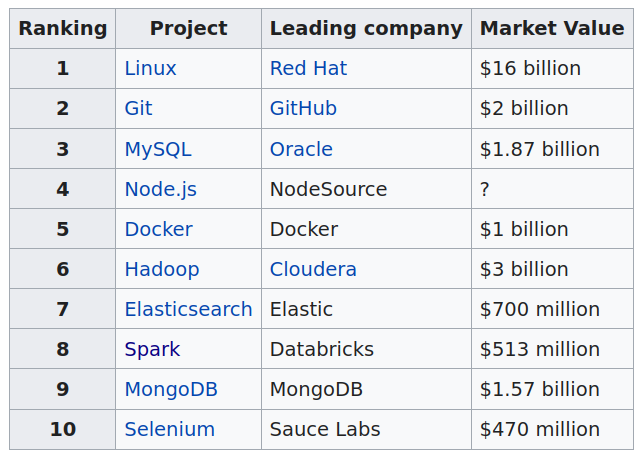
\includegraphics[width=0.9\textwidth]{img/oss}

{\noindent\tiny Battery Open Source Software Index (BOSS), 2017 \\\href{https://en.wikipedia.org/wiki/Open_source}{https://en.wikipedia.org/wiki/Open\_source}\\\href{https://computersweden.idg.se/2.2683/1.703485/microsoft-kop-github}{https://computersweden.idg.se/2.2683/1.703485/microsoft-kop-github}} 

\end{Slide}

\begin{Slide}{OSS \& samhällsutvecklingen}
\begin{itemize}
\item Operativsystem
\item Desktop-appar, Webb-appar
\item Infrastruktur: språk, verktyg, CI, ''Molnet'' (serverhallar, datalagring)
\item AI, ML
\item Tvärindustriell utveckling\\(energi, transport, finans, media, ...)
\item Den offentliga sektorn, \Alert{demokratin}\\ public money $\Rightarrow$ open source
\end{itemize}
\end{Slide}

\begin{Slide}{Hur välja OSS?}
\begin{itemize}
\item Koden
\begin{itemize}
\item api-kvalitet 
\item dokumentation
\item mognad
\item aktivitet
\end{itemize}  
\item Gemenskapen \hfill \emph{community health}
\begin{itemize}
\item ledning \hfill \emph{governance}
\item vem är aktiv med vad
\item code-of-conduct 
\end{itemize}  
\item Affärsmodellen
\begin{itemize}
\item licensmodell (pryl, system, tjänst)
\item differentierande eller stödjande
\end{itemize}  
\end{itemize}  
\end{Slide}

\begin{Slide}{Hur få inflytande över OSS?}
\begin{itemize}
  \item meritokrati
  \item bidra aktivt, bygga förtroende
  \item skapa allianser
  \item samarbeta \emph{och} konkurrera samtidigt
\end{itemize}  
\end{Slide}


\begin{Slide}{Hur få inflytande över OSS?}
\begin{itemize}
  \item meritokrati
  \item bidra aktivt, bygga förtroende
  \item skapa allianser
  \item samarbeta \emph{och} konkurrera samtidigt
\end{itemize}  

\vspace{1em}
{
\small \emph{Johan Linåker, Björn Regnell}:\\ ''\textbf{What to share, when, and where:} balancing the objectives and complexities of open source software contributions'' \\Empirical Software Engineering, (2020) 25:3799-3840 } \\ {\tiny \url{https://doi.org/10.1007/s10664-020-09855-2}}
\end{Slide}



\begin{Slide}{Läs artikel [OSS]}

{\small
Walt Scacchi: ''Understanding requirements for open source software.'' \textit{Design requirements engineering: A ten-year perspective. Springer, 2009. 467-494. }}
\begin{itemize}
  \item En studie av 5 OSS-projekt
  \item Kravhantering i OSS-projekt är ofta informell
  \item Transparenta diskussioner
  \item Öppen infrastruktur där samarbete och externa kodbidrag uppmuntras
  \item Kraven finns ofta i ärendehanterings-\\system kopplad till kodlagringsplatsen
  \item Många intressenter med egna agendor
\end{itemize}  

\end{Slide}


% \begin{Slide}{Utveckla en företagsstrategi för att bidra till öppen källkod}
% \begin{itemize}\small
%   \item[] ''\textbf{What to share, when, and where:}\\balancing the objectives and complexities of open source software contributions''
%   \item[] \emph{Linåker, J. \& Regnell, B.} 
%   \item[] \emph{\tiny Empirical Software Engineering, (2020) 25:3799-3840} 
%   \item[] {\tiny \url{https://doi.org/10.1007/s10664-020-09855-2}}
% \end{itemize}  
% \end{Slide}

% \Img{-0.65cm}{0.65}{img/oss-strategy}

% \Subsection{\texttt{cs.lth.se/krav}}  

% \Subsection{Avslutning}

% \begin{Slide}{TODO}
% \begin{itemize}
%   \item 
% \end{itemize}  
% \end{Slide}

\end{document}
